\section{La régression logistique}
\label{chap4.section6}
De par le fait qu'ils sont caractérisés par une ensemble fixe de paramètres (généralement égal au nombre de prédicateurs + 1 bias), les modèles de régression linéaire sont obligés de construire une hypothèse forte sur la fonction inconnue qui a génère les données. Parce que contrairement aux modèles non paramètriques comme les arbres de décisions, ils n'ont pas la capacité de changer de forme ou de grandir pour s'adapter parfaitement à l'ensemble d'entraînement, donc ils doivent faire des compromis pour trouver les meilleurs approximations des valeurs de poids et du bias qui minimise les pertes pour tous les exemples d'entraînement.

Cette particularité qui est censé être une contrainte de base s'avère finalement être la meilleure solution face au sur-ajustement. En effet ces modèles sont beaucoup moins sensible à ce problème, tout en faisant des prédictions correctes la plupart du temps. On veut pouvoir mettre ce type de modèle au service des problèmes de classification également, il y'a donc deux possibilités majeures qui s'offre à nous: le \textbf{seuillage} ou la conversion de prédictions réelle continues en \textbf{probabilité}.

Avec la regression logistique on choisit la deuxième option afin de pouvoir faire de cette conversion une partie intégrante du modèle. Plus exactement, la régression logistique est une modification de la régression linéaire parfaitement pensée pour les problèmes de classification binaire (comme prédire les défaut de paiement). L'idée est de prendre un modèle de régression linéaire et de l'équiper d'une fonction qui puisse transformer la sortie \(\hat{y}_j = b + \Sigma_i w_i \cdot x_{j,i}\) en la probabilité que l'exemple \(x_j\) appartienne à la classe positif. Cette fonction est connue sous le nom de fonction \textbf{sigmoid} et est définie par: \[Sigmoid(z) = \frac{1}{1 + e^{-z}}\] C'est bien la fonction de la fin de l'algorithme \ref{chap4.sec4.sub1}. Vous pouvez remarquez que quelque soit la valeur de \(z\) les valeurs de cette fonction sont dans l'intervalle \(]0, 1[\).

En grosso modo, l'idée est de modifier légèrement un modèle de régression linéaire de manière à ce que les prédictions du modèle soit désormais sous la forme \(Sigmoid(z)\) où \(z = \hat{y}_j = b + \Sigma_i w_i \cdot x_{j,i}\) représentant la probabilité que l'exemple \(x_j\) appartienne à la classe positif (représentée par 1) qui dans notre cas signifie que le client fera défaut sur son prêt. La figure \ref{fig:fig8} montre l'effet de la fonction sigmoid sur les prédictions du modèle de régression et comment ces probabilités sont typiquement interprêtées.

\begin{figure}
    \centering
    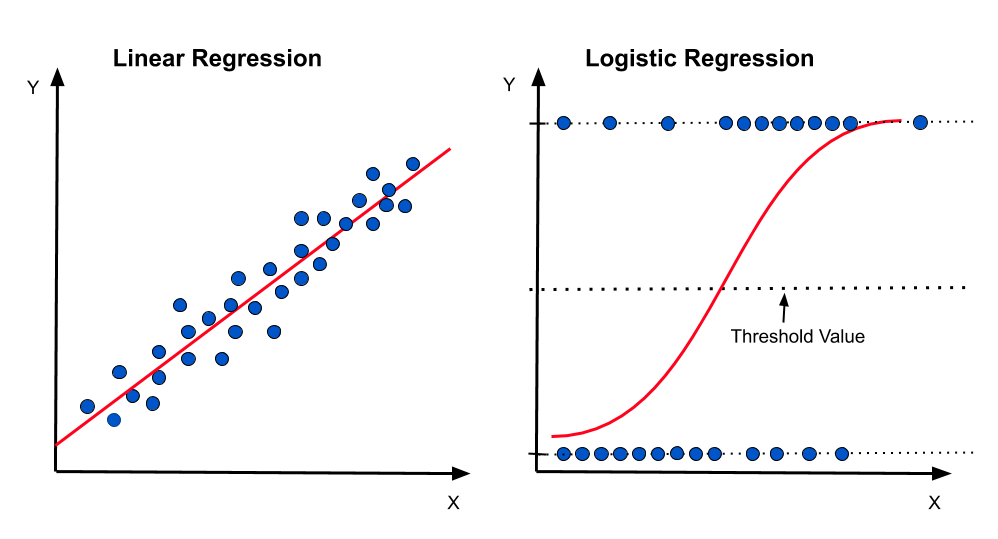
\includegraphics[width=0.75\linewidth]{images/logitReg.png}
    \caption{Visualisation d'un modèle de régression logistique simple}
    \label{fig:fig8}
\end{figure}

\subsection{Algorithme (Descente de gradient)}
\label{chap4.sec6.sub1}
Le concept et l'algorithme de descente de gradient utilisé pour entraîner le modèle reste fondamentalement le même. Il y'a juste une petite nouvouté, puisque maintenant la prédiction du modèle n'est plus donnée directement par \(\hat{y}_j = b + \Sigma_i w_i \cdot x_{j,i}\) mais plutôt par \(Sigmoid(\hat{y}_j)\) on va avoir besoin d'une étape supplémentaire pour trouver le gradient de la fonction de perte par rapport aux différents poids et au bias parce que la fonction de coût \(L2\) qu'on va encore utilisée pour l'illustration elle est toujours en fonction de \(\hat{y}_j\) comme toute autre fonction de coût en soit. Ce qui nous amène au calcul suivant:

\begin{itemize}
    \item Pour un exemple d’entraînment \(x_j\) et un certain \(w_i\), poids du \(i\)ème attribut de \(x_j\) on a donc: \[\frac{\partial}{\partial w_i} L2 = \frac{\partial L2}{\partial Sigmoid(\hat{y}_j)} \cdot \frac{\partial Sigmoid(\hat{y}_j)}{\partial \hat{y}_j} \cdot \frac{\partial \hat{y}_j}{\partial w_i}\]
    \item Pour le bias on a: \[\frac{\partial}{\partial b} L2 = \frac{\partial L2}{\partial Sigmoid(\hat{y}_j)} \cdot \frac{\partial Sigmoid(\hat{y}_j)}{\partial \hat{y}_j} \cdot \frac{\partial \hat{y}_j}{\partial b}\]
\end{itemize}

Avec les démonstrations de la section \ref{chap4.sec5.sub2} on sait que:  \[\frac{\partial L2}{\partial Sigmoid(\hat{y}_j)} = \frac{\partial}{\partial Sigmoid(\hat{y}_j)} (y_j - Sigmoid(\hat{y}_j))^2 = -2(y_j - Sigmoid(\hat{y}_j))\]
\[\frac{\partial \hat{y}_j}{\partial w_i} = \frac{\partial}{\partial w_i} (b + w_i \cdot x_{j,i}) = x_{j,i}\]
\[\frac{\partial \hat{y}_j}{\partial b} = \frac{\partial}{\partial b} (b + w_i \cdot x_{j,i}) = 1\]

Il ne reste donc plus qu'à dériver la fonction sigmoid par rapport à \(\hat{y}_j\), on obtient donc: \[(Sigmoid(\hat{y}_j))' = (\frac{1}{1 + e^{-\hat{y}_j}})' = \frac{-(-e^{-\hat{y}_j})}{(1 + e^{-\hat{y}_j})^2} = \frac{e^{-\hat{y}_j}}{(1 + e^{-\hat{y}_j})^2}\]

Au final on obtient:

\begin{itemize}
    \item Pour un exemple d’entraînment \(x_j\) et un certain \(w_i\), poids du \(i\)ème attribut de \(x_j\): \[\frac{\partial}{\partial w_i} L2 = -2(y_j - Sigmoid(\hat{y}_j)) \cdot \frac{e^{-\hat{y}_j}}{(1 + e^{-\hat{y}_j})^2} \cdot x_{j,i}\]
    \item Pour le bias: \[\frac{\partial}{\partial b} L2 = -2(y_j - Sigmoid(\hat{y}_j)) \cdot \frac{e^{-\hat{y}_j}}{(1 + e^{-\hat{y}_j})^2}\]
\end{itemize}

L'algorithme de descente de gradient reste exactement le même et les mêmes concepts s'applique. Ce qui est très intéressant avec les nouveaux modèles et démonstrations qu'on voit depuis le section \ref{chap4.section5} c'est qu'on peut remarquer que ces concepts et algorithmes peuvent se généraliser à d'autres fonctions et problèmes. Donc il est techniquement possible de remplacer la fonction \(L2\) et la fonction \(Sigmoid\) avec n'importe quelle autre fonction différentiable. Cela a permit le développement de d'autres algorithmes comme les réseaux de neuronnes artificiels.

\subsection{Implémentation}
\label{chap4.sec6.sub2}
Mon implémentation de la régression logistique est assez « peu conventionnelle » on va dire, puisque je l'ai implémenté avec keras qui est un framework (une structure) pour l'apprentissage profond normalement (\cite{chollet2015keras}). Cela a donné un modèle avec des particularités qu'on associe typiquement aux réseaux de neuronnes, par exemple la descente de gradient est éffectuée par l'algorithme du \textbf{Moment adaptatif (AdaM)} qui est une version légèrement modifiée de l'algorithme de descente de gradient ordianaire décrit dans la section \ref{chap4.sec5.sub2}; de plus la mise à jour des paramètres se fait par lot, c'est-à-dire que les gradients sont accumulés et la descente se fait pour un lot à la fois, qui est une matrice de \(M\) exemples d'entraînement sur \(N\) au total au lieu de le faire pour chaque exemple individuellement ou pour une grande matrice de tout l'ensemble comme je l'avais précédemment évoqué. Ceci étant dit le fonctionnement du modèle est conceptuellement identique à celui d'un modèle de regression logistique et peut donc être considéré comme tel.

La raison pour laquelle j'ai décidé d'implémenter la régression logistique comme ceci est de faciliter la transition vers les réseaux de neuronnes dans ce document et pour ceux qui liront les codes.

Mon implémentation utilise aussi une fonction de coût différente de \(L2\) qui est pensée particulièrement pour les problèmes de classification et classification binaire notamment. C'est la fonction de \textbf{cross-entropie binaire} ou log-loss définie par: \[LogLoss = - [y_j \cdot log(p_j) + (1 − y_j)\cdot log(1−p_j)]\] où \(p_j = Sigmoid(\hat{y}_j)\) et donc la forme complète est la somme normalisée des pertes: \[LogLoss = - \frac{1}{N} \Sigma_j^N [y_j \cdot log(p_j) + (1 − y_j)\cdot log(1−p_j)]\] où \(N\) est le nombre d'exemple. De par son expression cette fonction de perte atteint sa valeur maximal quand \(y_j\) est trop différent de \(p_j\), une manière de pénaliser plus lourdement le modèle quand il a gravement tort et donc d'avoir des gradients plus grands pour rémedier à ça.

Le modèle a donc été entraîner sur ces bases là pour sept (07) époques sur des lots de 64 exemples et avec un taux d'apprentissage de 0,001 (\cite{diarra2024notebooks}).